\documentclass{article}
\textheight 23.5cm \textwidth 15.8cm
%\leftskip -1cm
\topmargin -1.5cm \oddsidemargin 0.3cm \evensidemargin -0.3cm
%\documentclass[final]{siamltex}

\usepackage{verbatim}
\usepackage{fancyhdr}
\usepackage{amssymb,ctex}
\usepackage{mathrsfs}
\usepackage{latexsym,amsmath,amssymb,amsfonts,epsfig,graphicx,cite,psfrag}
\usepackage{eepic,color,colordvi,amscd}
\usepackage{enumerate}
\usepackage{enumitem}
\usepackage{booktabs}
\usepackage{graphicx}
\usepackage{float}
\usepackage{wrapfig}
\usepackage{multirow}
\usepackage{subfigure}
\usepackage{diagbox}
\usepackage{wasysym}

\title{USTC\_CG HW8 Shader}
\author{张继耀,PB20000204}

\begin{document}
	\maketitle
	
	\tableofcontents
	
	\section {问题介绍}
	\subsection{主要目的}
		\begin{itemize}
		\item 实现 normal map 和 displacement map
	\end{itemize}

	\begin{itemize}
	\item 利用 displacement map 在 vertex shader 中进行简单降噪
\end{itemize}

	\begin{itemize}
	\item 实现点光源阴影(可选)
\end{itemize}

	
	
	\section{算法设计}
	
	\subsection{法向贴图}
			\begin{figure}[H]
		\begin{center}
			
			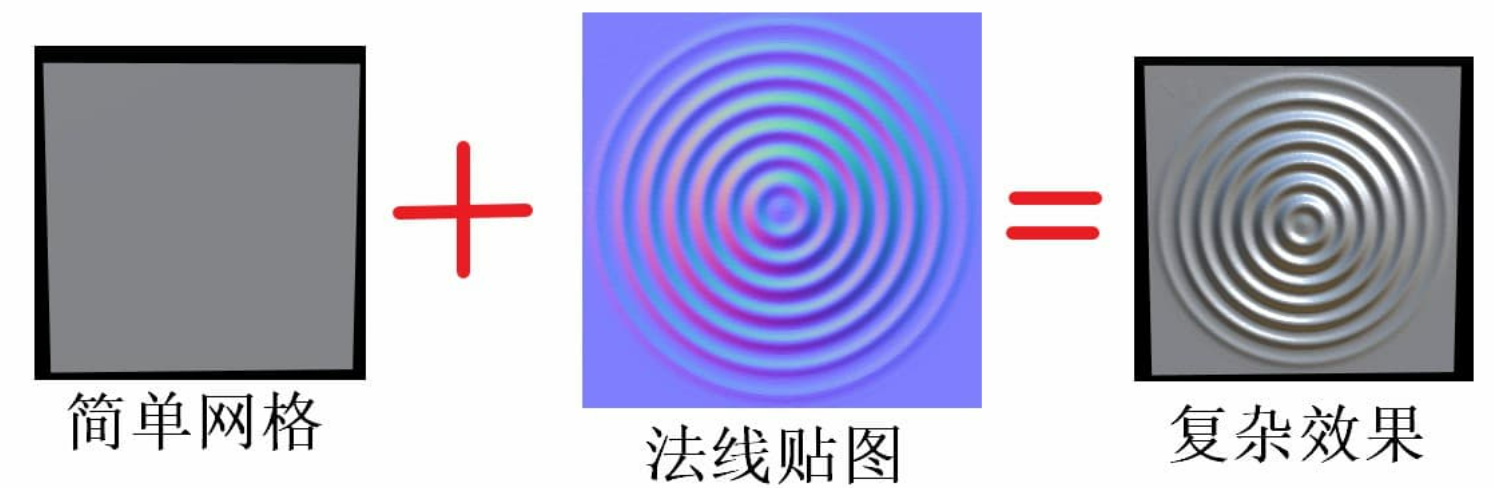
\includegraphics[width=15cm,height=4.5cm]{faxiang}
			
			\caption{法向贴图}	\label{faxiang.label}
		\end{center}
	\end{figure}
	
	在现实世界中,物体的表面往往不是光滑的,可能是粗糙的、凹凸不平的,有很多丰富的细节。从光照算法的视角考虑,为了使渲染的效果更加真实,我们可以改变它的法向向量。这就是法向贴图的原理。
		\begin{figure}[H]
		\begin{center}
			
			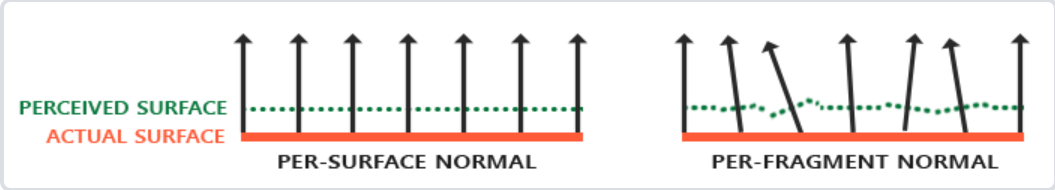
\includegraphics[width=15cm,height=3.5cm]{yuanli}
			
		 \caption{实现原理}	\label{jiemian.label}
		\end{center}
	\end{figure}
   如上图所示,如果每个fragment都是用自己不同的法线的话,我们就可以根据表面细微的细节对法线向量进行改变;这样就会获得一种表面看起来要复杂得多的幻觉:
   		\begin{figure}[H]
   	\begin{center}
   		
   		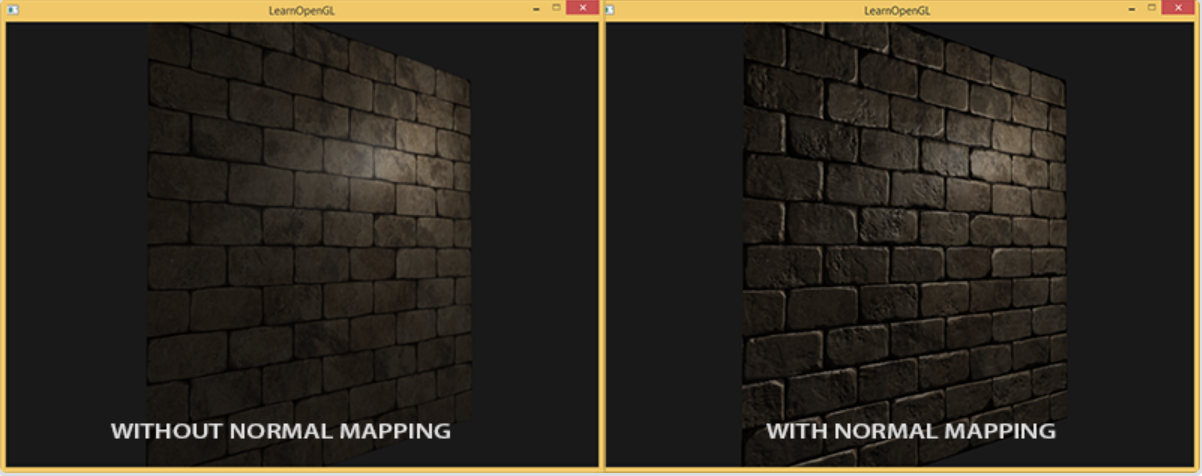
\includegraphics[width=15cm,height=5.5cm]{duibi}
   		
   		\caption{对比效果}	\label{duibi.label}
   	\end{center}
   \end{figure}

  法向贴图就是这样通过改变原法向来达到渲染效果的。但还有一个问题是:法向贴图中储存的所有法向向量都是指向正z方向的。对于不同的表面,这样产生的光照肯定是不对的。我们的解决方案是:用一个变换矩阵(TBN矩阵)将它转换到世界坐标下即可。
  
  只需在顶点着色器中计算该点的TBN矩阵;然后在片段着色器中把切线坐标空间的向量转换到时间坐标空间,再进行后续操作即可。
	
	\subsection{置换贴图}
	
		\begin{figure}[H]
		\begin{center}
			
			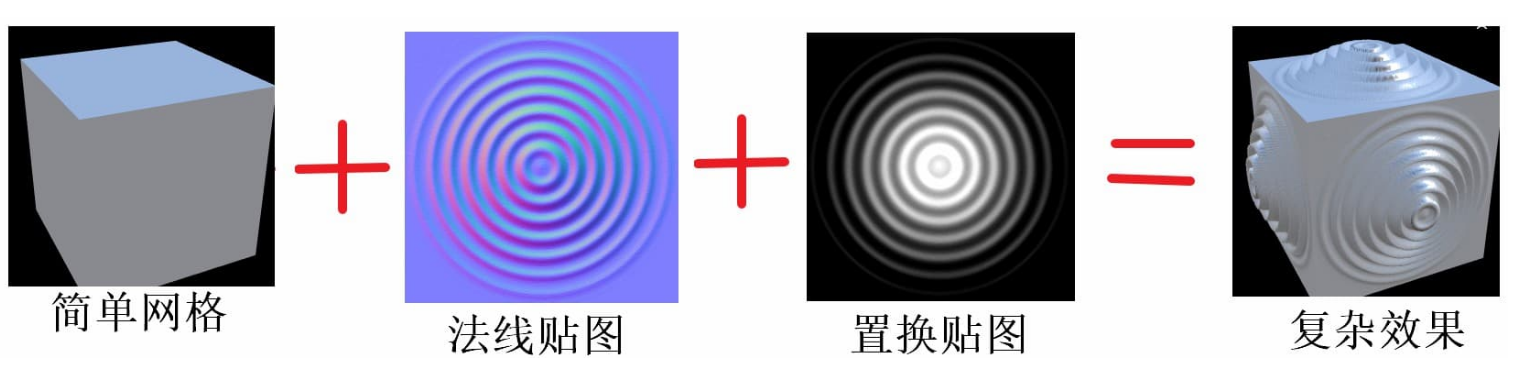
\includegraphics[width=17cm,height=4cm]{zhihuan}
			
			\caption{置换贴图}	\label{zhihuan.label}
		\end{center}
	\end{figure}
     置换贴图则是对点的实际坐标进行沿法向的偏移,直接改变顶点的位置,其中0(黑色)代表不动,1(白色)表示沿着法向偏移。
     
     具体的偏移程度是由像素值和系数$\lambda$来决定的,像素值是$[0,1]$中的浮点数,作变换
         $$ displacement = \lambda *(bias+scale*PixelValue) $$
      可以将$[0,1]$映为任意区间$[bias,bias+scale]$,再乘上系数$\lambda$。具体流程如下:
      \begin{itemize}
      	\item 在顶点着色器中从置换贴图中采样,进行相应的变换得到相应变化量displacement;
      \end{itemize}
     \begin{itemize}
  	\item 将该点的坐标沿法向偏移相应的变化量
  	    $$  P_i^{'}=P_i+displacement*n_i $$
  	    
  	    再用新的坐标参与后续运算。
    \end{itemize}

    \begin{itemize}
	\item 由于置换贴图只改变了顶点的位置,不改变顶点的法向,所以在使用时要加上对应的法向贴图。
    \end{itemize}

   
		\subsection{置换贴图去噪}
	 对一个给定的网格,虽然每个顶点被加了随机噪声,但法线还是用了原本的。所以含噪声模型在渲染的不同主要体现在纹理的扭曲和边缘的凹凸不平上。只要用置换贴图将每个顶点的位置进行合理的偏移,就能达到去噪的效果。
	 
	 步骤如下:
	   \begin{itemize}
	 	\item 计算每个顶点的偏移量
	 	    $$  \delta_i=p_i-\frac{1}{\left| N_j \right|}\sum_{j\in N(i)}p_j   $$
	 \end{itemize}
 
    \begin{itemize}
 	\item 将偏移量投影到法向上
 	$$  \overline{\delta_i}= \left<\delta_i,n_i \right>n_i $$
 \end{itemize}

     \begin{itemize}
    	\item 对每一个顶点进行偏移
    	$$  \overline{p_i}= p_i - \lambda\overline{\delta_i} = p_i - \lambda  \left<\delta_i,n_i \right>n_i    $$
    \end{itemize}

 \begin{itemize}
	\item 将$\left<\delta_i,n_i \right>$插值存到置换贴图中,注意设置$bias$和$scale$将值变换到0和1之间。
\end{itemize}
	
	   \subsection{点光源阴影}
	   \subsubsection{阴影映射}
	 阴影是光线被阻挡的结果;当一个光源的光线由于其他物体的阻挡不能够达到一个物体的表面的时候,那么这个物体就在阴影中了。阴影能够使场景看起来真实得多。
	 \begin{figure}[H]
	 	\begin{center}
	 		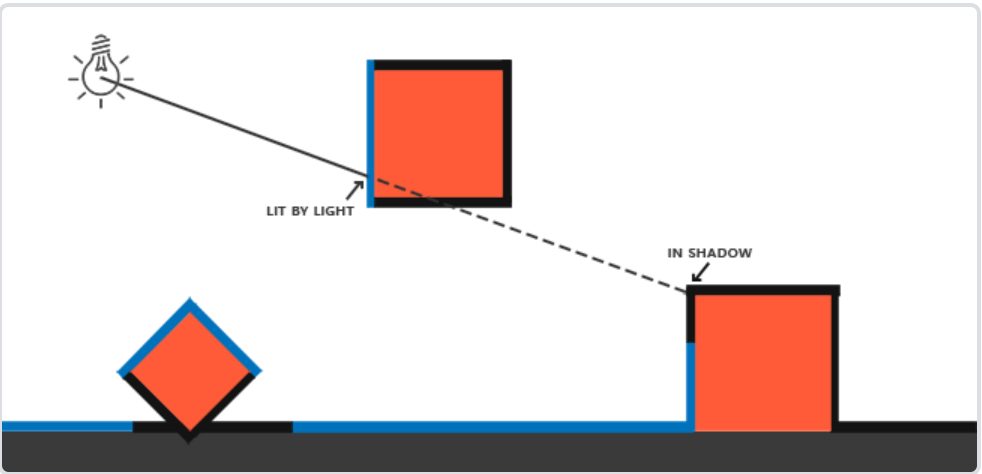
\includegraphics[width=17cm,height=6.5cm]{shadow mapping}
	 		\caption{阴影映射}	\label{yingshe.label}
	 	\end{center}
	 \end{figure}
 
  \begin{itemize}
 	\item 以光的位置为视角进行渲染,能看到的东西都将被点亮,看不见的则位于阴影之中。如上图所示,假设有一个地板,在光源和它之间有一个大盒子。从光源处向光线方向看去,可以看到这个盒子,但看不到地板的一部分,这部分就应该在阴影中了。
 \end{itemize}

  \begin{itemize}
	\item 如果绘制一条从光源出发,到达最右边盒子上的一个片段上的线段或射线,那么射线将先击中悬浮
	的盒子,随后才会到达最右侧的盒子。结果就是悬浮的盒子被照亮,而最右侧的盒子将处于阴影之
	中。
\end{itemize}

  \begin{itemize}
	\item 得到射线第一次击中的那个物体,然后用这个最近点和射线上其他点进行对比。然后测试一下看看
	射线上的其他点是否比最近点更远,如果是的话,这个点就在阴影中。
\end{itemize}

  \begin{itemize}
	\item 从光源的透视图来渲染场景,并把深度值的结果储存到纹理中。我们管储存在纹理中的所有这些深度值,叫做深度贴图(depth map)或阴影贴图。
\end{itemize}
	 \begin{figure}[H]
		\begin{center}
			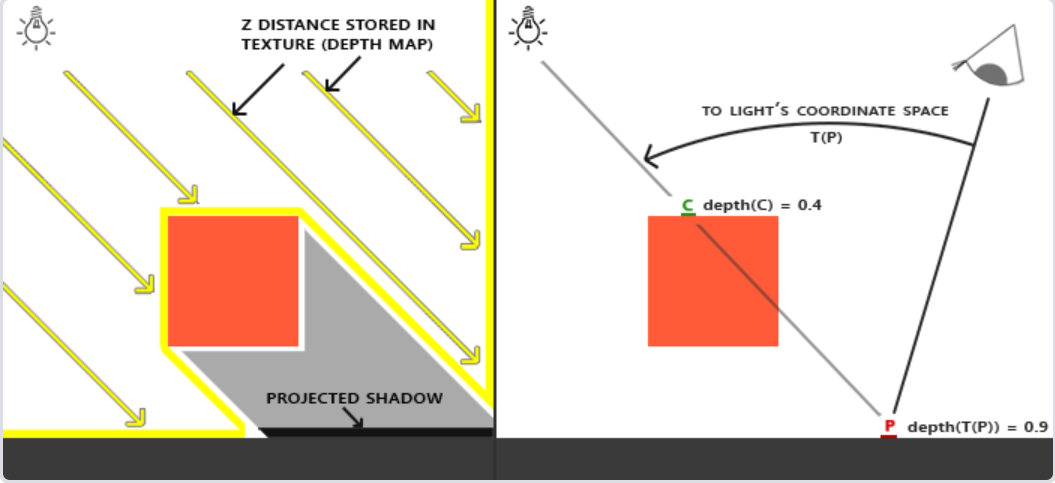
\includegraphics[width=15cm,height=6cm]{depth map}
			\caption{深度贴图}	\label{shendu.label}
		\end{center}
	\end{figure}
通过储存到深度贴图中的深度值,我们就能找到最近点,用以决定片段是否在阴影中。我们使用一个来自光源的视图和投影矩阵来渲染场景就能创建一个深度贴图。这个投影和视图矩阵结合在一起成为一个$T$变换,它可以将任何三维位置转变到光源的可见坐标空间。

	\subsubsection{深度贴图}
	  \begin{itemize}
		\item 深度贴图就是从光的透视图里渲染的深度纹理,用它计算阴影。
	\end{itemize}

  \begin{itemize}
	\item 为光源使用正交投影矩阵,同时为了创建一个视图矩阵来变换每个物体,把它们变换到从光源视角
	可见的空间中,使用look\_at函数;这次从光源的位置看向场景中央。二者相结合便得到了光空间的
	变换矩阵lightSpaceMatrix,它将每个世界空间坐标变换到光源处所见到的那个空间。这个lightSpaceMatrix正是前面我们称为$T$的那个变换矩阵。
\end{itemize}

  \begin{itemize}
	\item 顶点着色器将一个单独模型的一个顶点,使用lightSpaceMatrix变换到光空间中。
\end{itemize}

	\subsubsection{渲染阴影}
	  \begin{itemize}
		\item 正确地生成深度贴图以后我们就可以开始生成阴影了。这段代码在片段着色器中执行,用来检验一个片段是否在阴影之中。
	\end{itemize}
	  \begin{itemize}
	\item 把光空间片段位置转换为裁切空间的标准化设备坐标,自己做透视除法。
\end{itemize}

  \begin{itemize}
	\item 有了这些投影坐标,我们就能从深度贴图中采样得到0到1的结果,从第一个渲染阶段的projCoords坐标直接对应于变换过的NDC坐标。我们将得到光的位置视野下最近的深度:
\end{itemize}

  \begin{itemize}
	\item 为了得到片段的当前深度,我们简单获取投影向量的z坐标,它等于来自光的透视视角的片段的深度。
\end{itemize}

  \begin{itemize}
	\item 实际的对比就是简单检查currentDepth是否高于closetDepth,如果是,那么片段就在阴影中。
\end{itemize}

	\subsubsection{阴影失真问题}
	
	上面得到的阴影映射还是有不真实的地方,我们需要对它做一些修正。
		 \begin{figure}[H]
		\begin{center}
			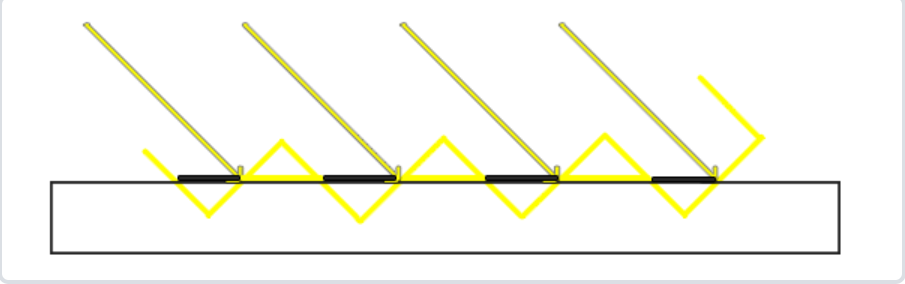
\includegraphics[width=15cm,height=4.5cm]{yinyingshizhen}
			\caption{阴影失真现象的原因}	\label{yinying.label}
		\end{center}
	\end{figure}

因为阴影贴图受限于分辨率,在距离光源比较远的情况下,多个片段可能从深度贴图的同一个值中去采样。图片每个斜坡代表深度贴图一个单独的纹理像素。你可以看到,多个片段从同一个深度值进行采样。

  解决方案:对表面的深度(深度贴图)做一个偏移量,这样片段就不会被错误地认为在表面之下了。
  
  	 \begin{figure}[H]
  	\begin{center}
  		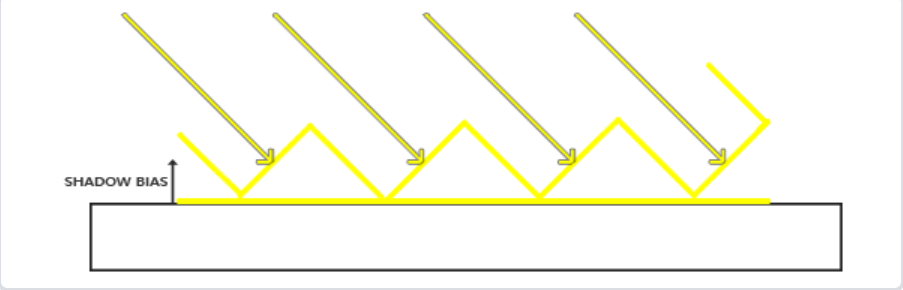
\includegraphics[width=15cm,height=4.5cm]{bias}
  		\caption{阴影偏移}	\label{pianyi.label}
  	\end{center}
  \end{figure}

	\subsubsection{悬浮}
	
	  \begin{itemize}
		\item 使用阴影偏移的一个缺点是你对物体的实际深度应用了平移。偏移有可能足够大,以至于可以看出阴影相对实际物体位置的偏移。
	\end{itemize}

	  \begin{itemize}
		\item 我们可以使用一个叫技巧解决大部分的Peter panning问题:当渲染深度贴图时候使用正面剔除(front face culling)
	\end{itemize}
	\subsubsection{采样过多}
	
		  \begin{itemize}
		\item 光的视锥不可见的区域一律被认为是处于阴影中,不管它真的处于阴影之中。出现这个状况是因为超出光的视锥的投影坐标比1.0大,这样采样的深度纹理就会超出他默认的0到1的范围。根据纹理环绕方式,我们将会得到不正确的深度结果,它不是基于真实的来自光源的深度值。
	\end{itemize}
	
	\begin{itemize}
		\item 解决这个问题也很简单,只要投影向量的z坐标大于1.0,我们就把shadow的值强制设为0.0:
	\end{itemize}
	
	\subsubsection{分辨率问题}
	
	  \begin{itemize}
		\item 因为深度贴图有一个固定的分辨率,多个片段对应于一个纹理像素。结果就是多个片段会从深度贴
		图的同一个深度值进行采样,这几个片段便得到的是同一个阴影,这就会产生锯齿边。
	\end{itemize}
	
	\begin{itemize}
		\item 从深度贴图中多次采样,每一次采样的纹理坐标都稍有不同。每个独立的样本可能在也可能不再阴
		影中。所有的次生结果接着结合在一起,进行平均化,就得到了柔和阴影。
	\end{itemize}
	
	
	\section{结果展示}
	
	\subsection{法向贴图和置换贴图}
	
\begin{figure}[H]
	\begin{center}
		
		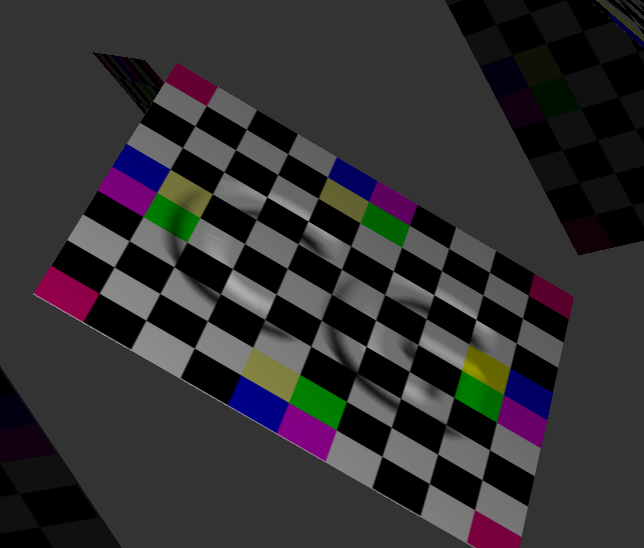
\includegraphics[width=7cm,height=5cm]{faxiang lizi}
		
		\caption{法向贴图} \label{faxiang lizi.label}
	\end{center}
\end{figure}

\begin{figure}[H]
	\begin{center}
		
		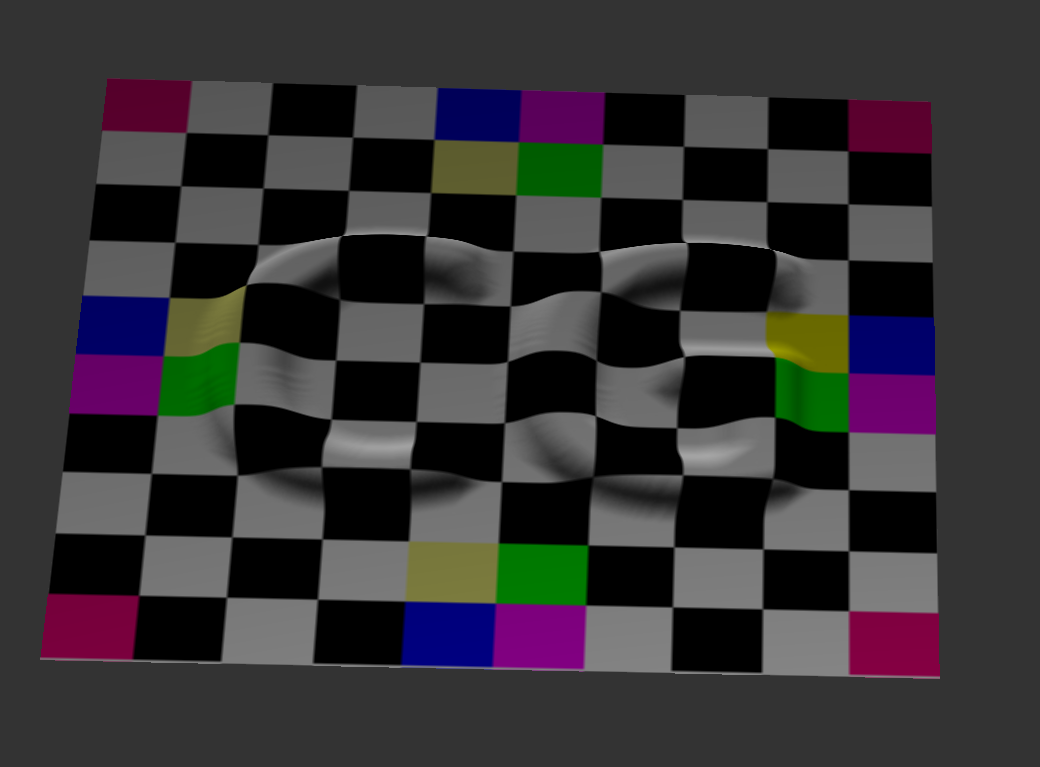
\includegraphics[width=7cm,height=5cm]{zhihuan lizi}
		
		\caption{置换贴图} \label{zhihuan lizi.label}
	\end{center}
\end{figure}

下面是一些使用不同背景的例子

\begin{figure}[H]
	\begin{center}
		
		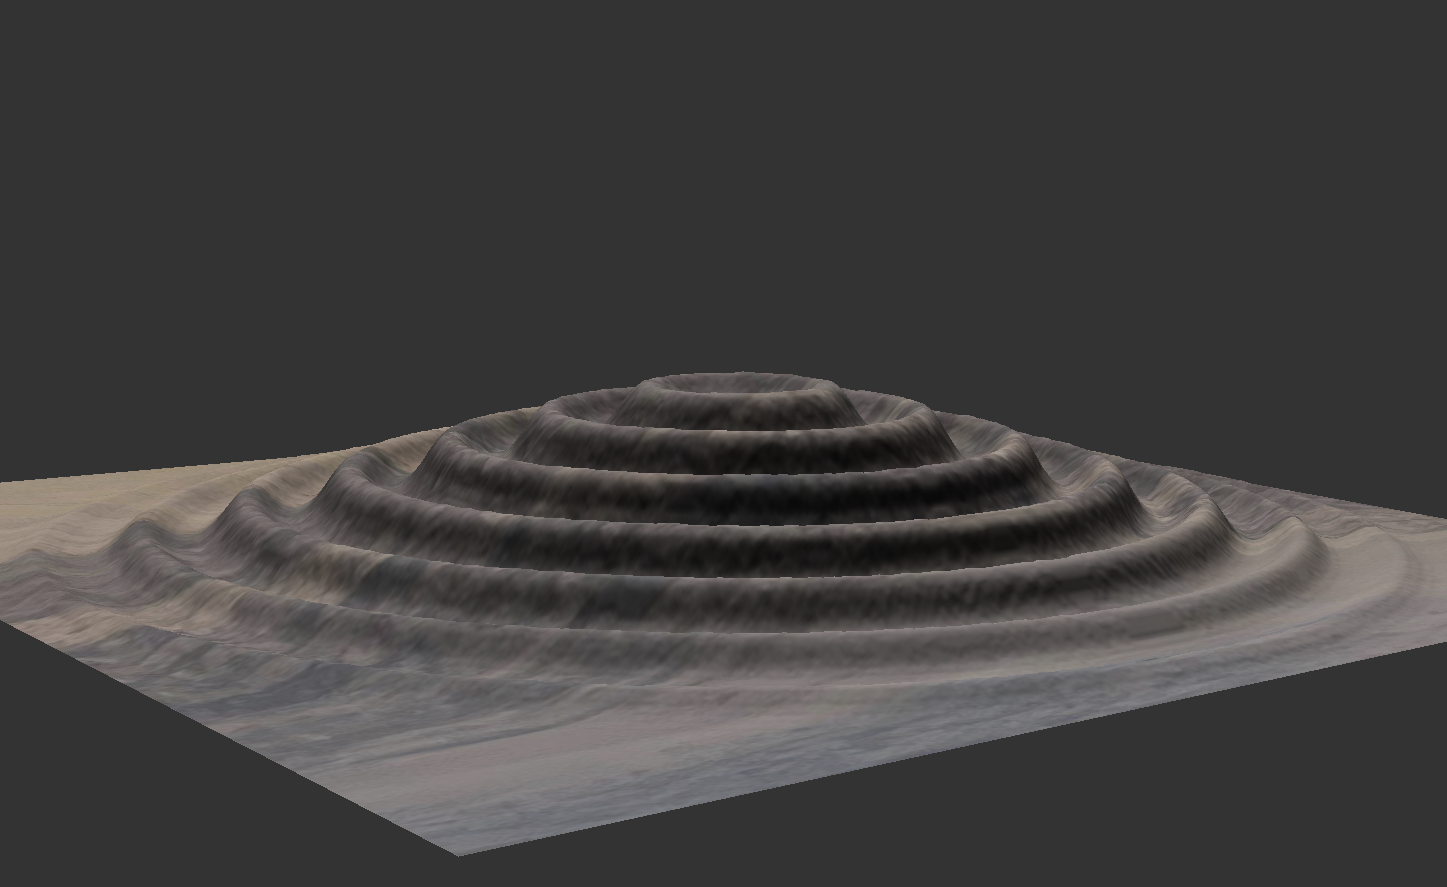
\includegraphics[width=7cm,height=5cm]{gebi0}
		
		\caption{沙漠} \label{lvzhou.label}
	\end{center}
\end{figure}



\begin{figure}[H]
	\begin{center}
		
		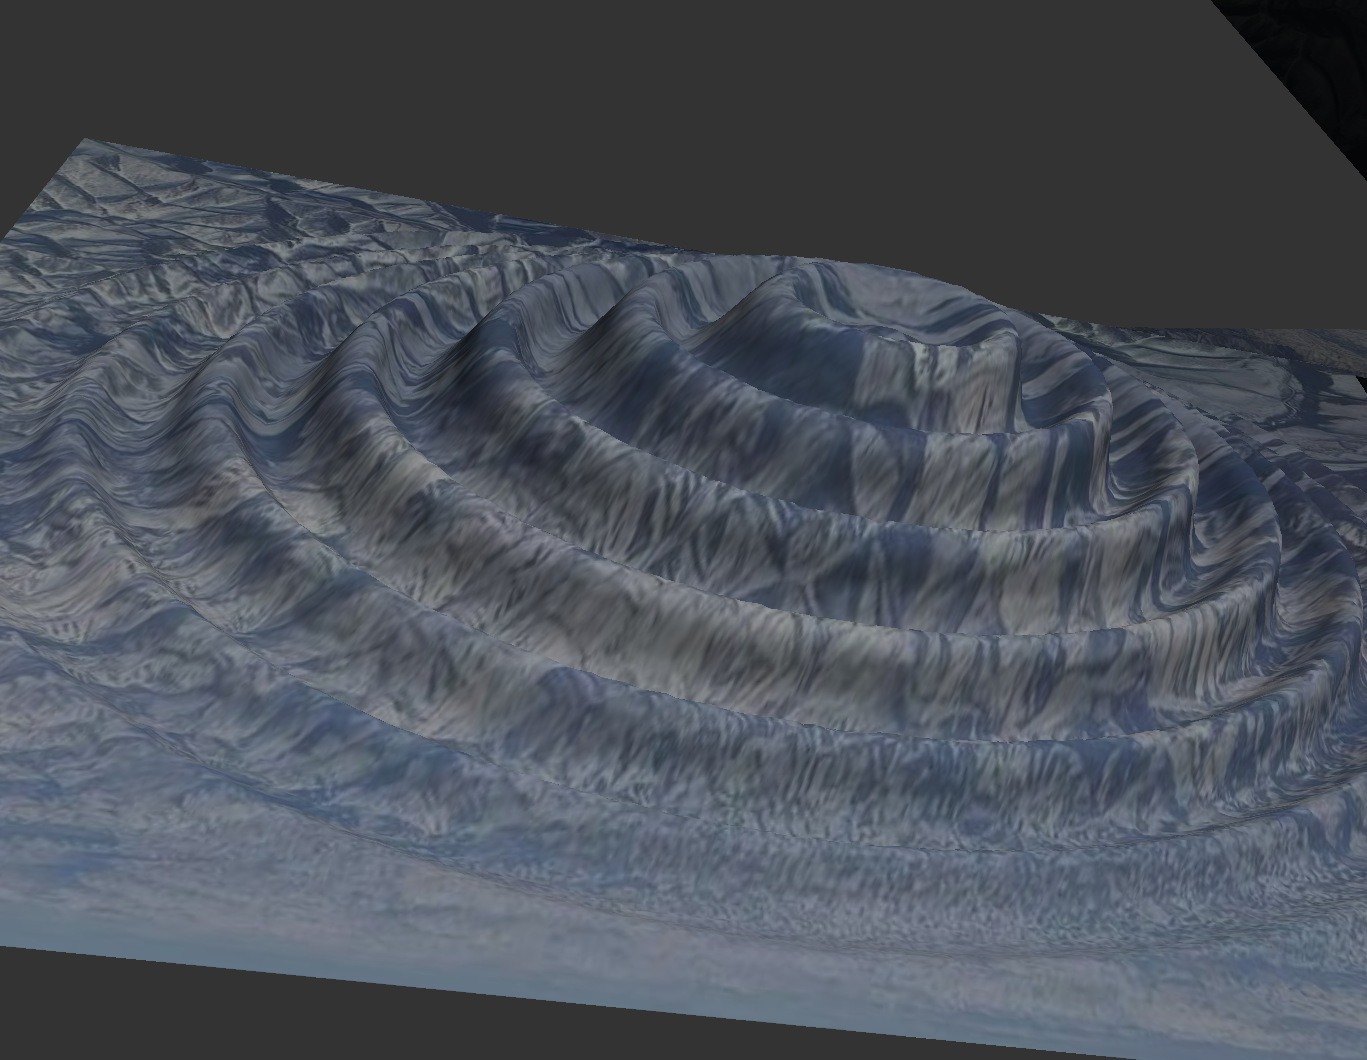
\includegraphics[width=7cm,height=5cm]{bing1}
		
		\caption{冰原} \label{bingyuan1.label}
	\end{center}
\end{figure}

   以及改变置换贴图中参数的取值时,得到的结果也是不同的。
   
   \begin{figure}[H]
   	\begin{center}
   		
   		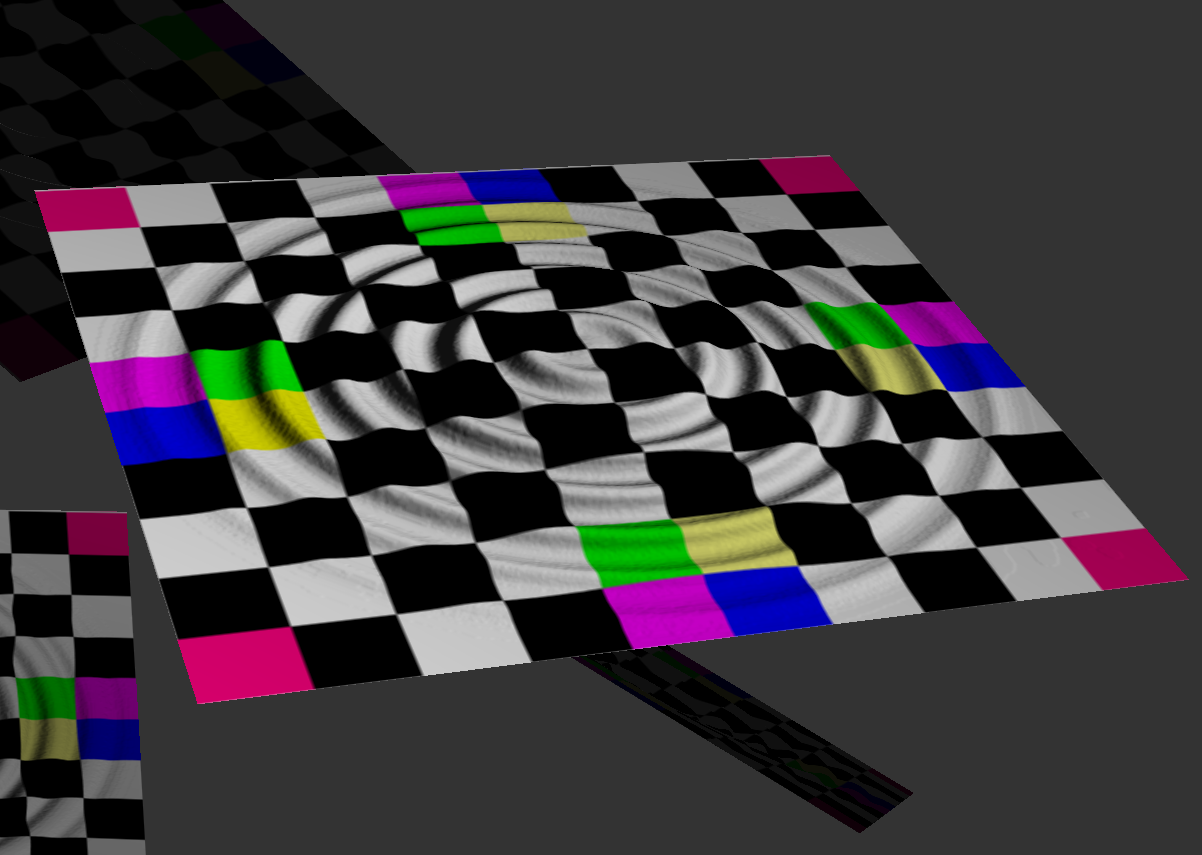
\includegraphics[width=7cm,height=5cm]{zhihuan 0 2}
   		
   		\caption{bias=0,scale=1} \label{zhihuan 0 2.label}
   	\end{center}
   \end{figure}

  \begin{figure}[H]
	\begin{center}
		
		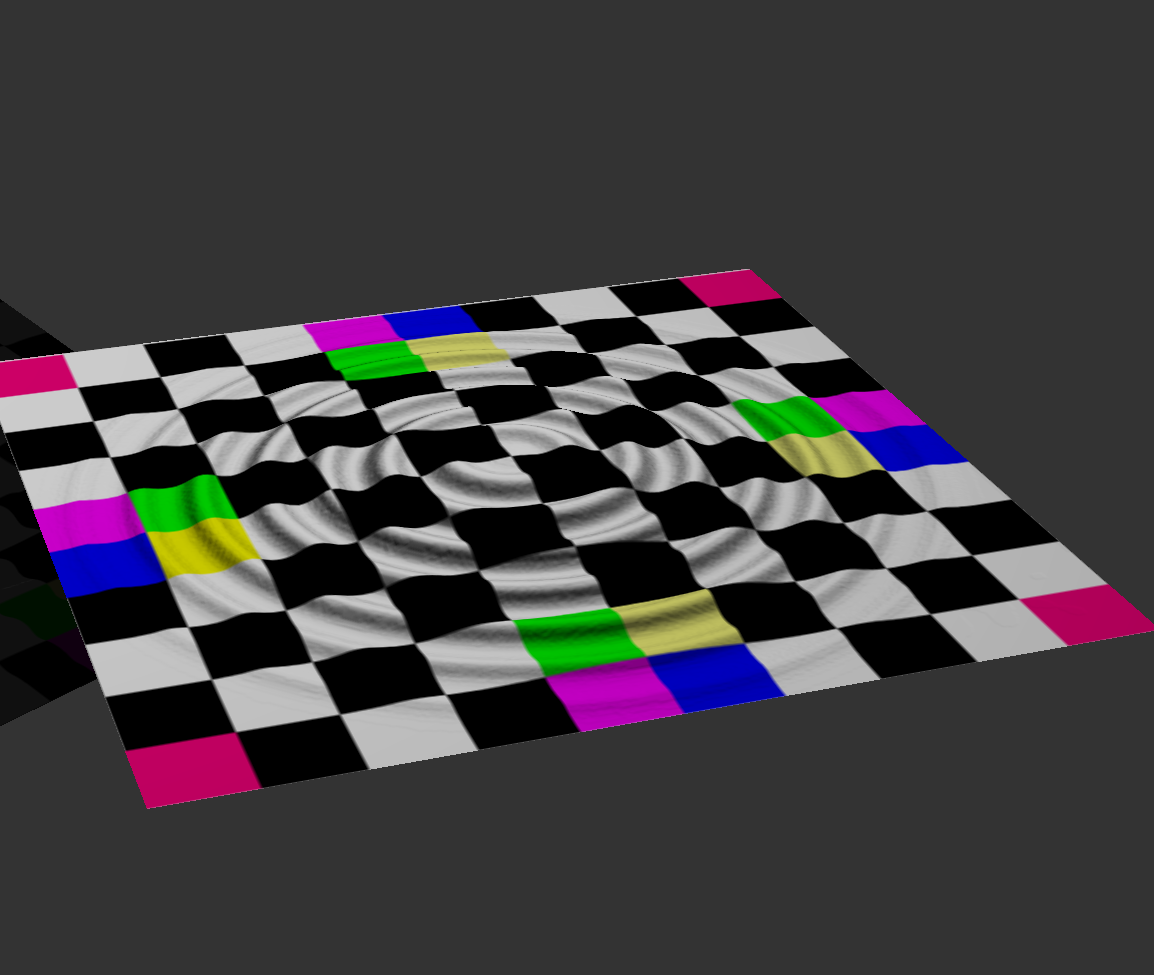
\includegraphics[width=7cm,height=5cm]{zhihuan -1 2}
		
		\caption{bias=-1,scale=2} \label{zhihuan -1 2.label}
	\end{center}
\end{figure}

  \begin{figure}[H]
	\begin{center}
		
		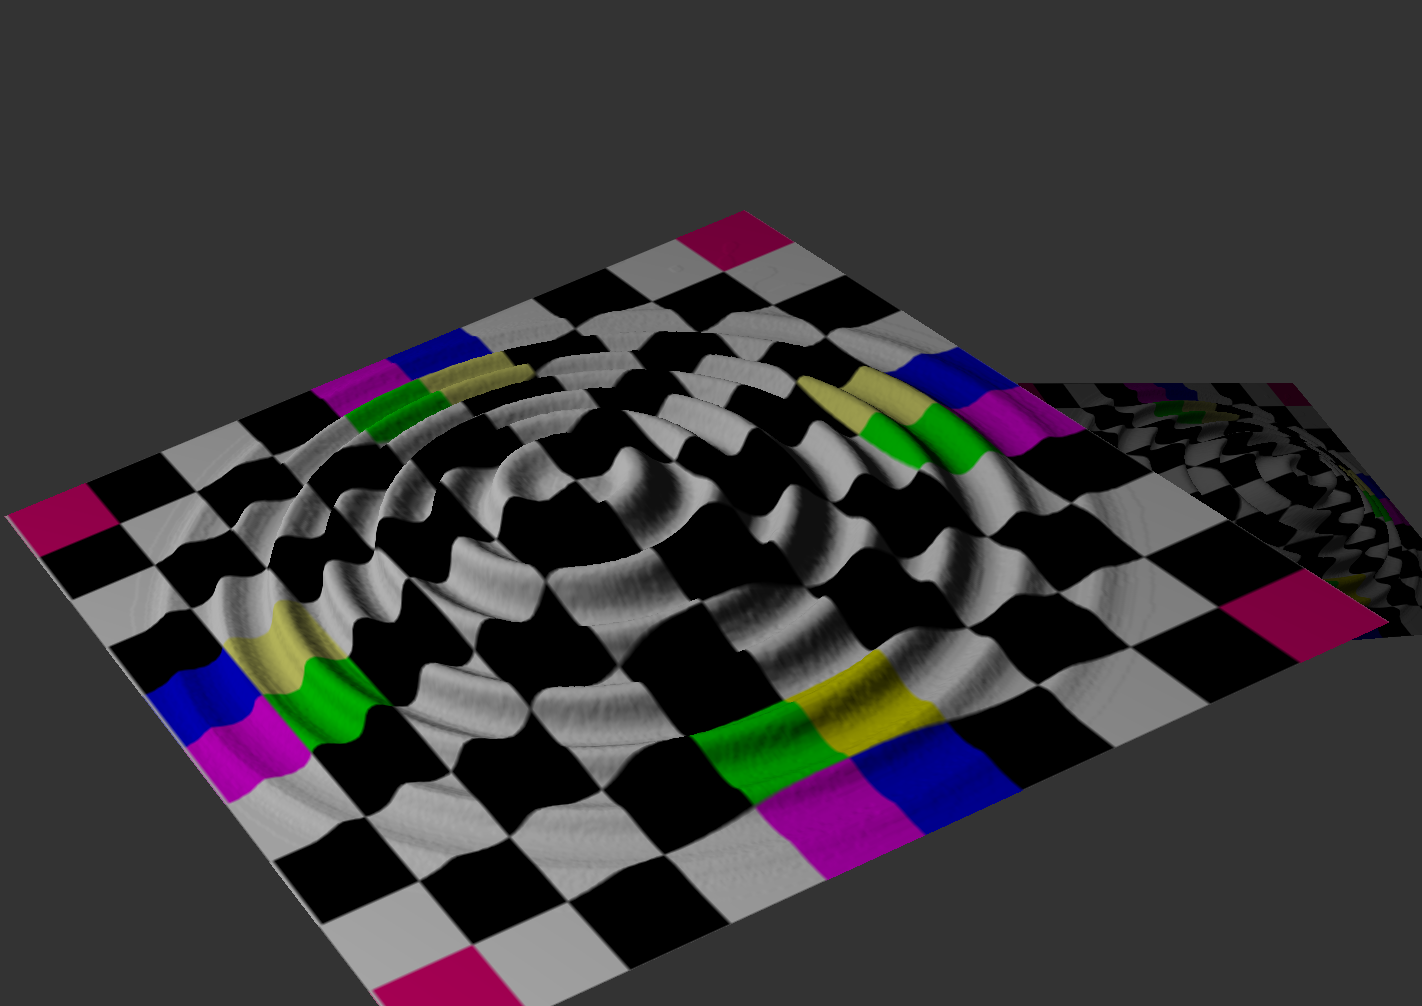
\includegraphics[width=7cm,height=5cm]{zhihuan -1 5}
		
		\caption{bias=-1,scale=5} \label{zhihuan -1 5.label}
	\end{center}
\end{figure}
	
	\subsection{使用置换贴图去噪}
	
	  \begin{figure}[H]
		\begin{center}
			
			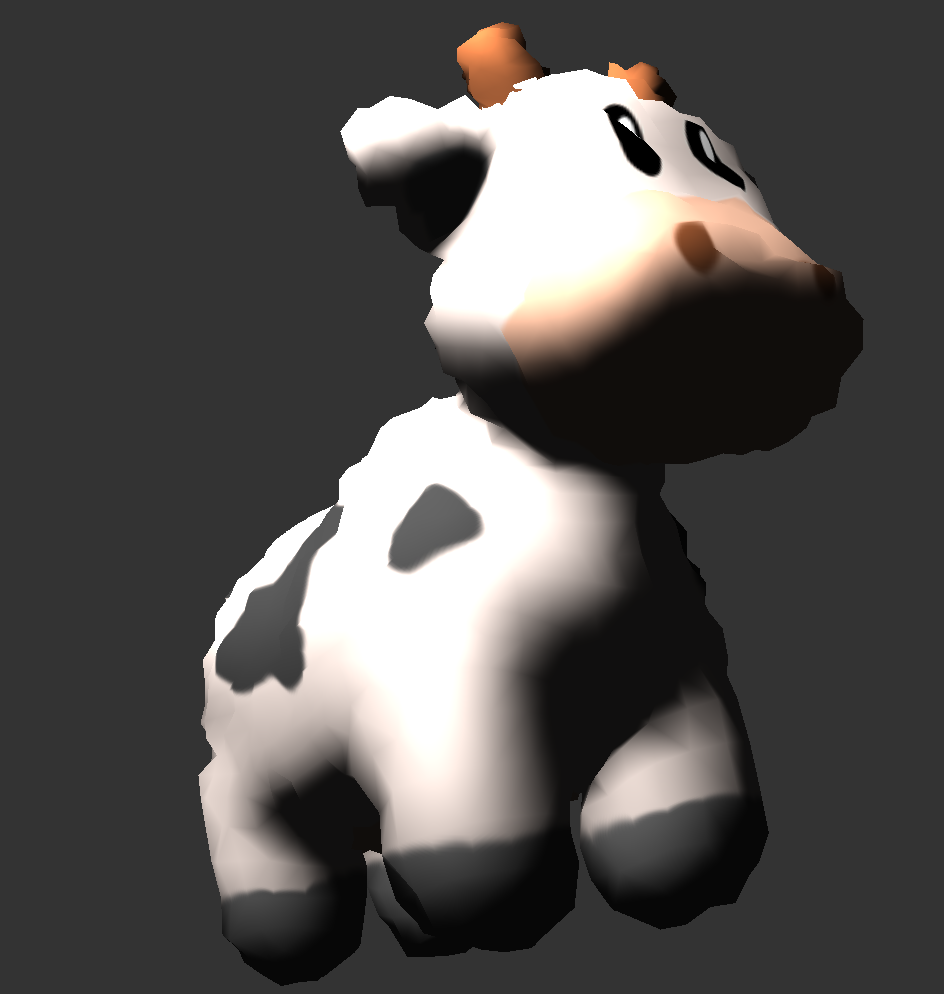
\includegraphics[width=7cm,height=5.5cm]{noise yuantu}
			
			\caption{带噪音的原图} \label{noiseyuan.label}
		\end{center}
	\end{figure}

	  \begin{figure}[H]
	\begin{center}
		
		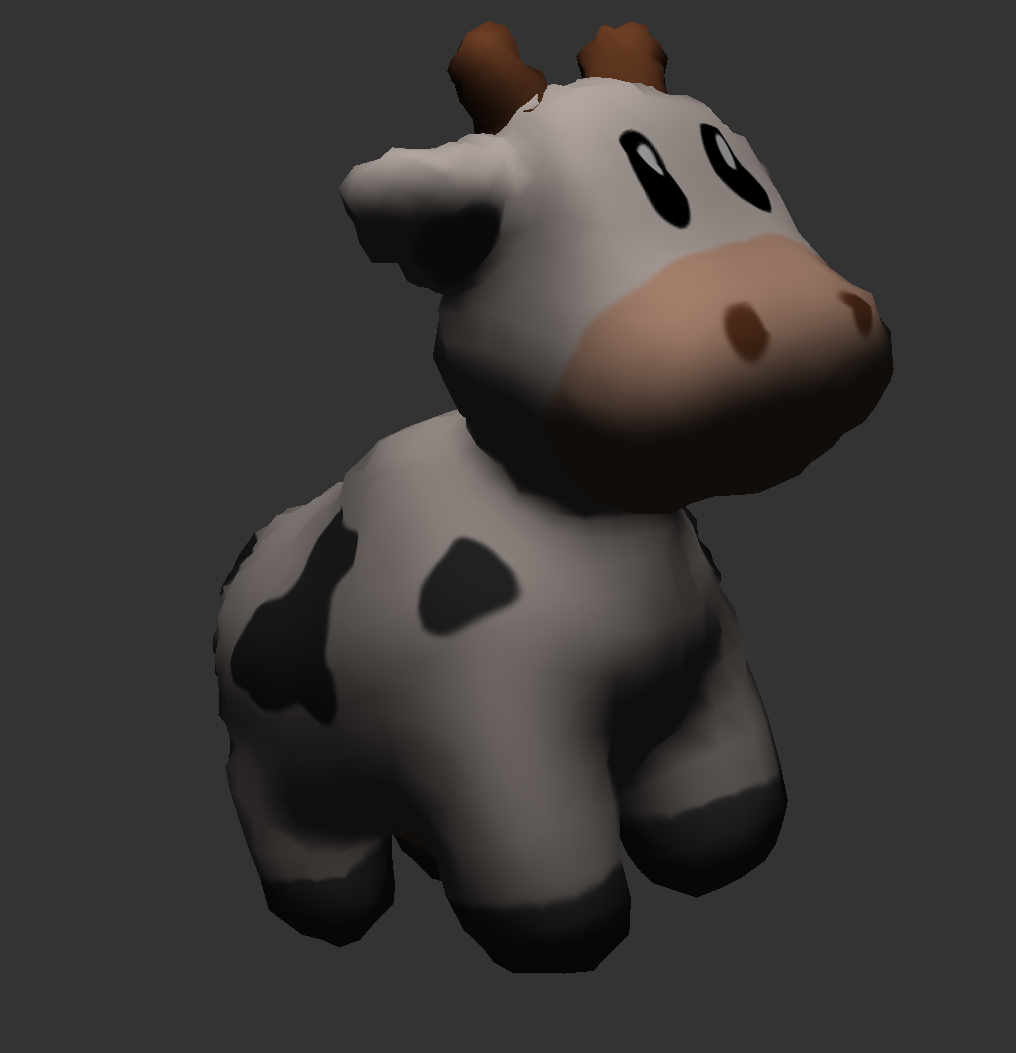
\includegraphics[width=7cm,height=5.5cm]{noise 0.3}
		
		\caption{$\lambda=0.3$的结果} \label{0.3.label}
	\end{center}
\end{figure}

	  \begin{figure}[H]
	\begin{center}
		
		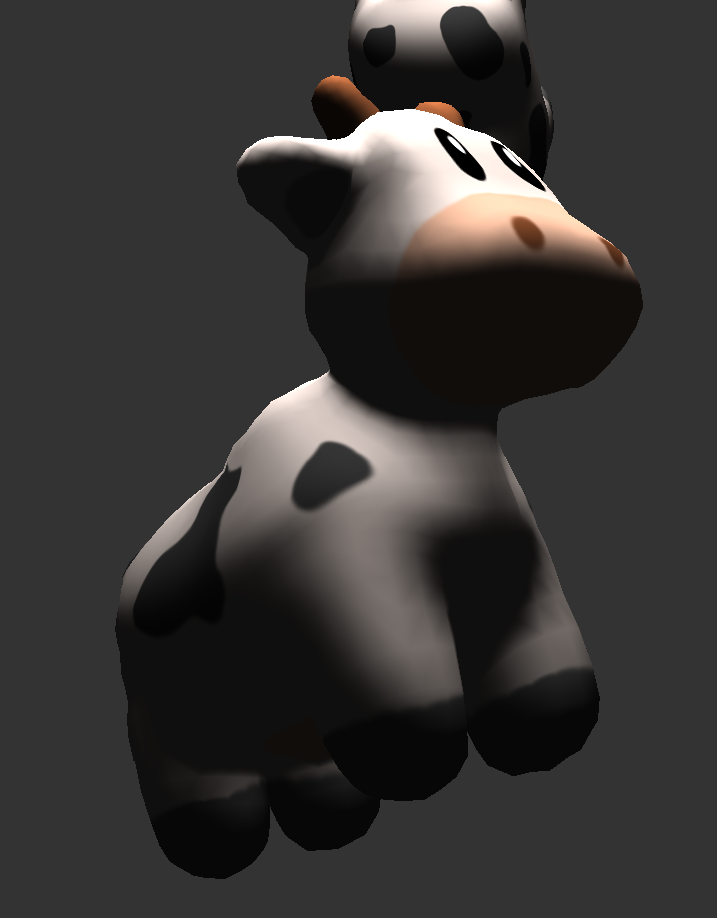
\includegraphics[width=7cm,height=5.5cm]{noise 0.7}
		
		\caption{$\lambda=0.7$的结果} \label{0.7.label}
	\end{center}
\end{figure}

	  \begin{figure}[H]
	\begin{center}
		
		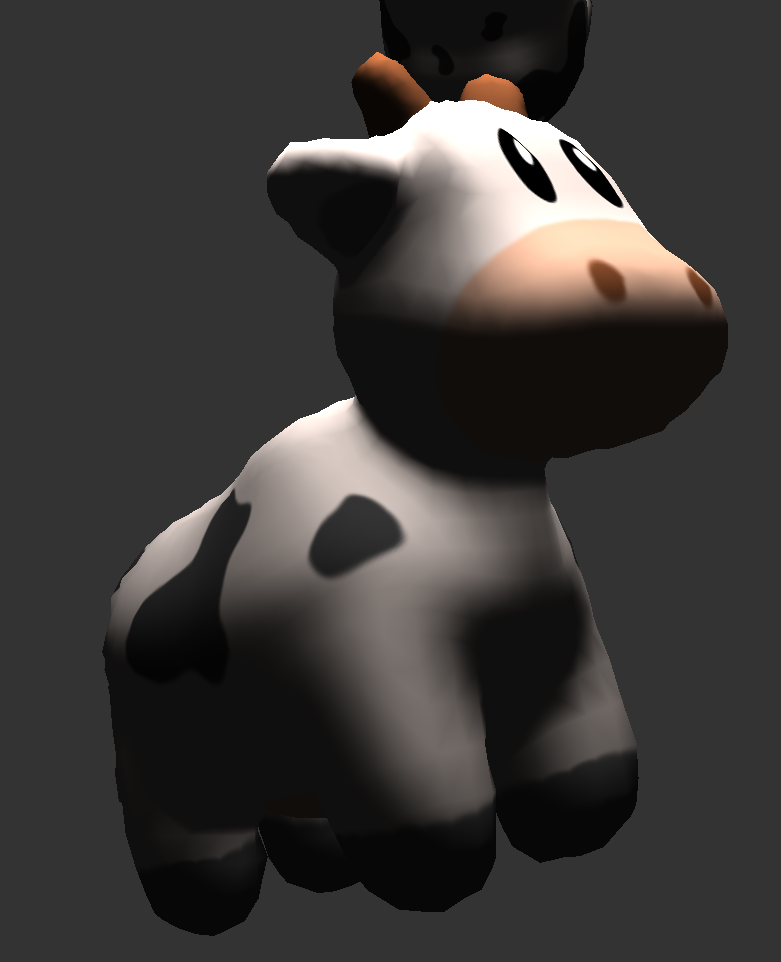
\includegraphics[width=7cm,height=5.5cm]{noise 1}
		
		\caption{$\lambda=1$的结果} \label{1.label}
	\end{center}
\end{figure}

  在修补噪声的过程中可能会产生缝隙,需要对这些点进行特殊处理,否则就会有如下的结果:
  
  	  \begin{figure}[H]
  	\begin{center}
  		
  		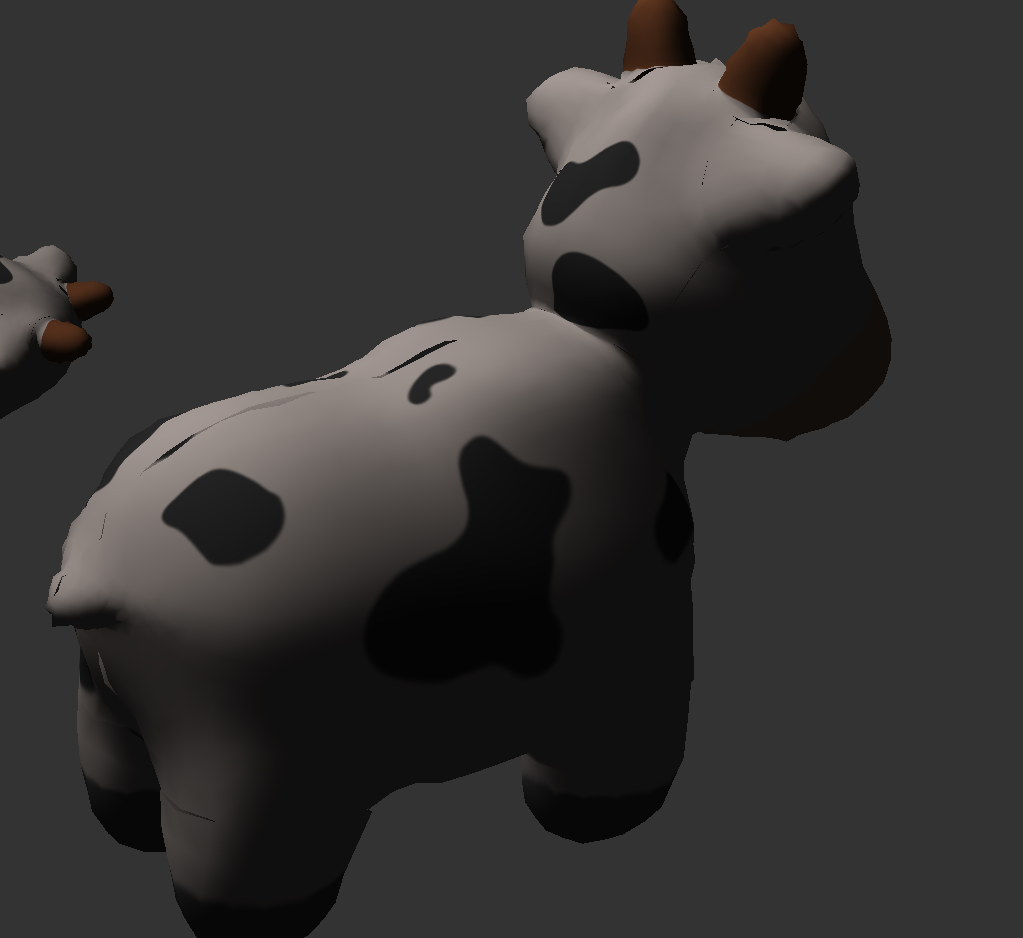
\includegraphics[width=7cm,height=5.5cm]{noise fengxi}
  		
  		\caption{未处理的结果} \label{feng.label}
  	\end{center}
  \end{figure}
	
	
	
	
	\section{总结与讨论}
	
	由于时间原因,点光源阴影没有来得及做了。感觉很多地方也不是很完善,也有很多可以改进的空间吧。但时间有限,只能这样了。。
	
	
\end{document}